\chapter{Image Processing and NDVI}
\label{sec:image_processing}
%SIFT, mapping, geotagging, alignment,\\

Once the images are undistorted as in Section \ref{sec:undistortion}, the images can be aligned using stereo-correspondence before an NDVI is performed.\\

A scale-invariant-feature-transform is applied to the images to align them using an affine transform. An NDVI calculation is applied to the matched images, with a floating point output image. A LUT colourmap is applied to visibly distinguish different areas and their meanings in the final image.

\section{Feature Detection}

There are different types of feature detection. 
\begin{itemize}
	\item Harris Corner Detection
	\item Shi-Tomasi Corner Detection
	\item SIFT (Scale-Invariant Feature Transform)
	\item SURF (Speeded-Up Robust Features)
	\item FAST (Features from Accelerated Segment Test)
	\item BRIEF (Binary Robust Independent Elementary Features)
	\item ORB (Oriented FAST and Rotated BRIEF)
%	\item BRISK, FREAK, KAZE, and AKAZE
\end{itemize}

There are also different types of feature matching.

\begin{itemize}
	\item Feature Matching + Homography to find Objects
	\item FLANN (Fast Library for Approximate Nearest Neighbors) based matcher
\end{itemize}

Harris Corner detection is useful for the chessboard calibration technique as in Section \ref{sec:cal_technique}. Shi-Tomasi improved the scoring function of Harris, but it is more appropriate for tracking. SIFT provides keypoints and descriptors. It also does not depend on the scale of a corner, unlike in Figure \ref{fig:sift_scale}. SURF is good at dealing with blurring and rotation, but not at handling viewpoint and illumination change as in SURF. FAST is better from a realtime, limited resource application point of view. Although it is several times faster than the other detectors, it is not robust against high levels of noise, and depends on a threshold. BRIEF is a quicker feature descriptor with lower memory usage, but feature detection such as SIFT, SURF is still needed. ORB is a good alternative to SIFT and SURF in performance, and is not patented.\\

\begin{figure}[H]
\centering
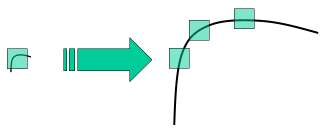
\includegraphics[scale=0.5]{images/sift_scale_invariant.jpg}
\caption{Harris corner detection on scaled corners. \cite{calib3d}}
\label{fig:sift_scale}
\end{figure}

\subsection{Feature matching}

SIFT returns landmark correspondence points between the stereo images.\\

It will then use brute-force feature matching, which calculates for each descriptor in the first image, the distance between it and all the features in the second image, returning the closest one. If the second closest corresponding point is within a threshold normalized distance of 0.8, according to David G. Lowe, it is discarded. The remaining candidates are filtered by geometric consensus.\\

%SURF is faster than SIFT, since it approximates the Laplacian of Gaussian with Box Filter instead of Difference of Gaussian.

\subsection{Homography}

Once the corresponding features are found, an affine transform matrix is found. For example, the estimated transformation matrix may be as in Equation \ref{eq:affine}.

\begin{equation}\label{eq:affine}
1.29837\cdot\begin{bmatrix}3 &3\end{bmatrix}
\begin{bmatrix}
1.00123 & 0.00442 & -10.778 \\ 0.11146\cdot10^-3 & 1.00130 & 19.372
\end{bmatrix}
\end{equation}

\section{Stitching and mapping}

A few images are stitched together to show proof-of-concept as in Figure \ref{fig:stitch_map}. A subset of about 100 images total are processed using MME \cite{mme}.

\begin{figure}[H]
\begin{subfigure}{0.5\textwidth}
\centering
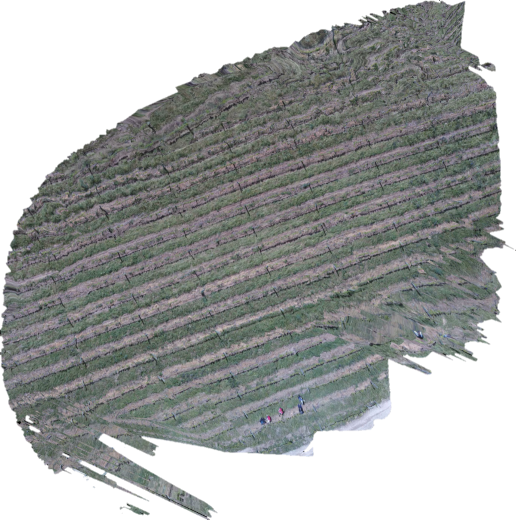
\includegraphics[scale=0.35]{images/map_rgb.png}
\caption{RGB map}
\end{subfigure}
\begin{subfigure}{0.5\textwidth}
\centering
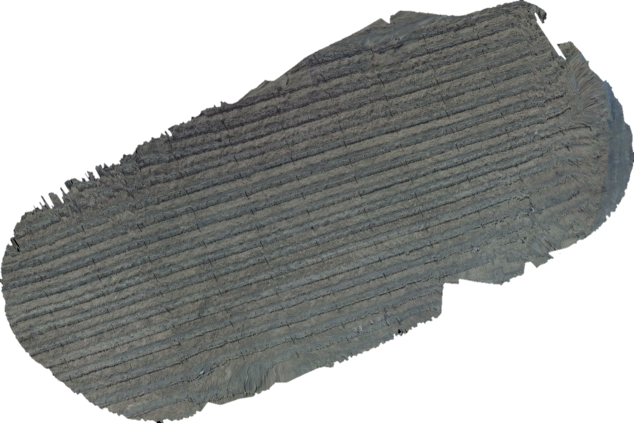
\includegraphics[scale=0.4]{images/map_ir.png}
\caption{NIR map}
\end{subfigure}
\caption{Maps processed using MME}
\label{fig:maps}
\end{figure}

The images are then co-registered using an algorithm called bUnwarpJ \cite{bunwarpj} as in Figure \ref{fig:stitch_map}. Image registration is based on elastic deformations represented by B-splines and pyramid coefficients. 

\begin{figure}[H]
\centering
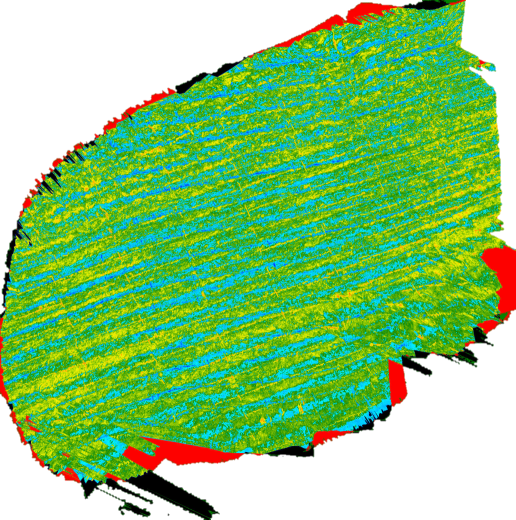
\includegraphics[scale=0.35]{images/map_ndvi.png}
\caption{NDVI performed using bUnwarpJ}
\label{fig:stitch_map}
\end{figure}

There does exist a larger map in Appendix \ref{app:ndvi_map}.

%\begin{figure}[H]
%\centering
%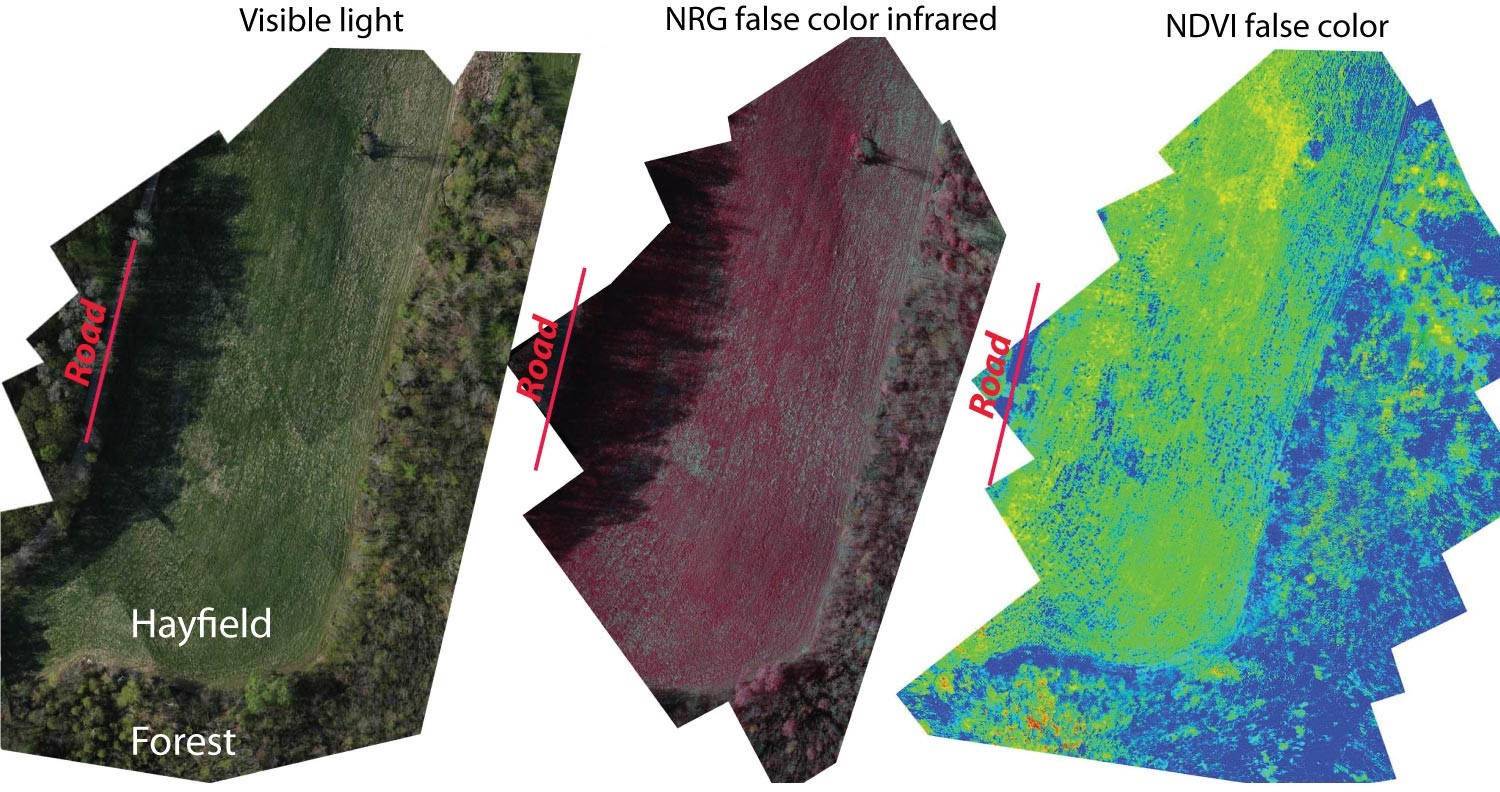
\includegraphics[scale=0.35]{images/ndvi_stitch_example.jpg}
%\caption{Photos stitched into a map}
%\label{fig:stitch_map}
%\end{figure}

\section{Calibration Plate}
\label{sec:cal_plate}

Moderate NDVI values apply to young/older (senescing) crops or grasslands and shrubs from about 0.2 to 0.5. Higher NDVI values from about 0.6 to 0.9 correspond to dense vegetation such as that found in forests or crops at their peak growth stage. \cite{ndvi_values}\\

NDVI values can drift due to sunlight, clouds, glare etc. The values have a scientific basis, and it would be good to calibrate the equipment before every flight, otherwise one can only retrieve relative NDVI values, which may not be very helpful over a long period of time. In general, the idea is to get consistent results, no matter the time or place.\\

A calibration plate from MicaSense was investigated. It has an NDVI value of 0.18. There is also a piece of red and blue paper, with the hope that it can be used as a cheap calibration plate.

\begin{figure}[H]
\begin{subfigure}{0.5\textwidth}
\centering
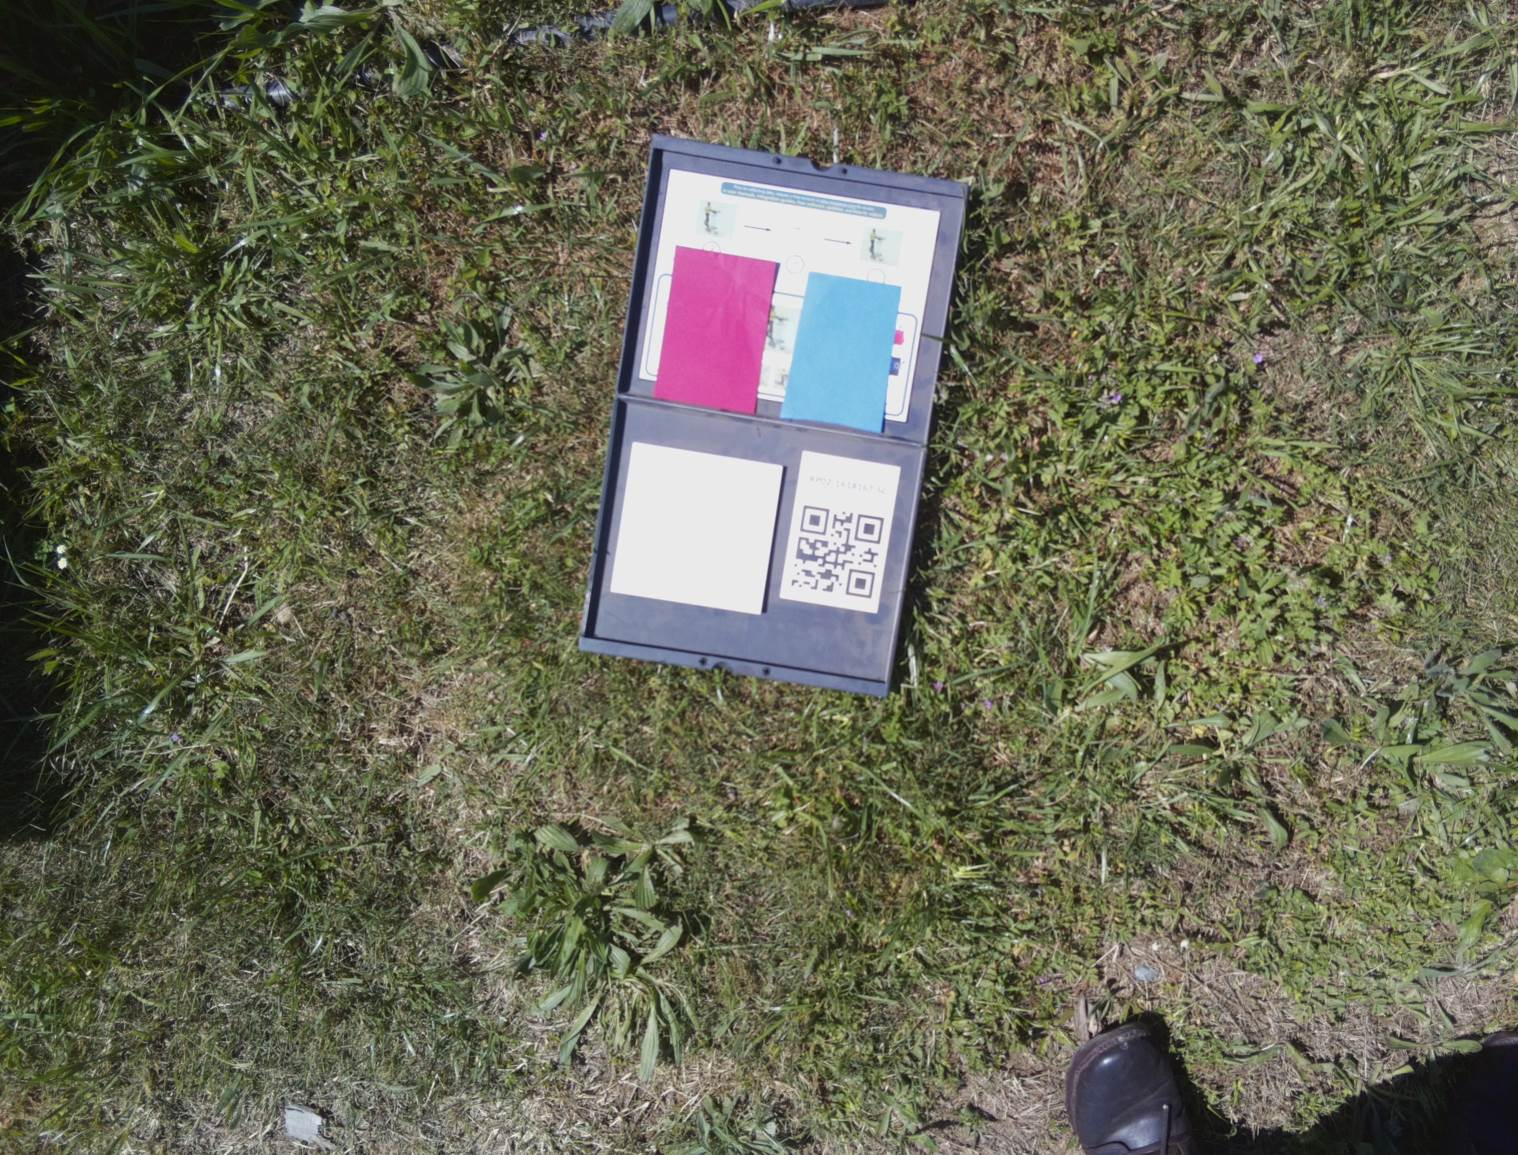
\includegraphics[scale=0.15]{images/rgb_cal.jpg}
\caption{RGB image}
\end{subfigure}
\begin{subfigure}{0.5\textwidth}
\centering
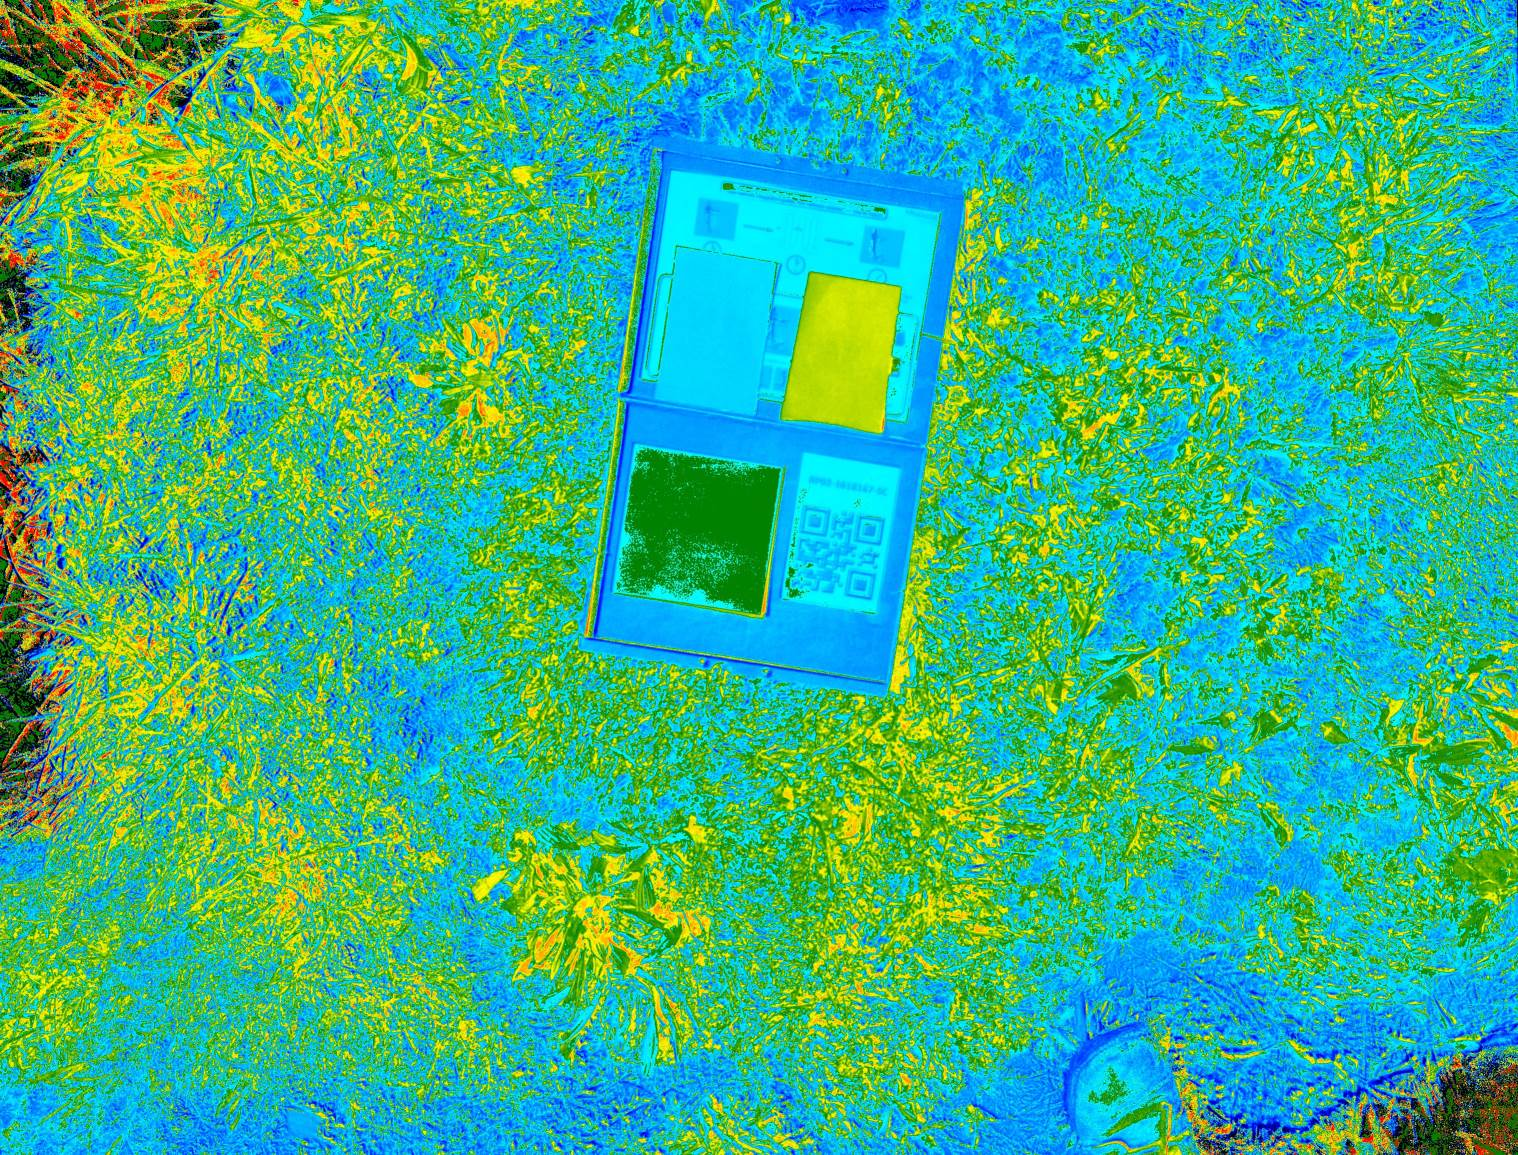
\includegraphics[scale=0.15]{images/ndvi_cal.jpg}
\caption{Processed NDVI image}
\end{subfigure}
\caption{Images take from Sony cameras used throughout project}
\label{fig:cal_plate}
\end{figure}

The plate has an NDVI value of -0.006, blue paper has 0.171, and red paper has 0.042.
%0,069
%0.073

\begin{figure}[H]
\begin{subfigure}{0.5\textwidth}
\centering
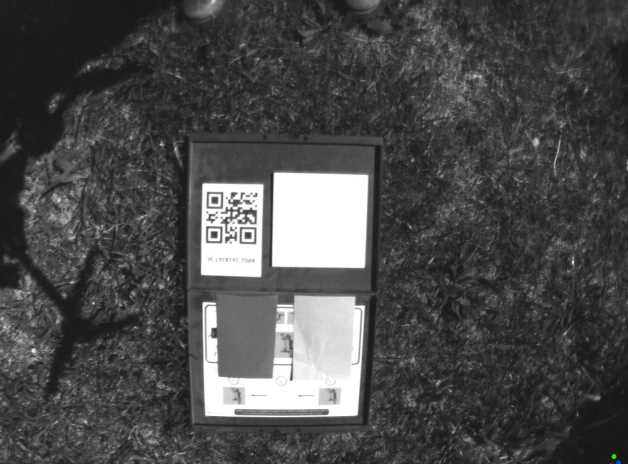
\includegraphics[scale=0.35]{images/sequoia_redcal.jpg}
\caption{Red (grayscale) image}
\end{subfigure}
\begin{subfigure}{0.5\textwidth}
\centering
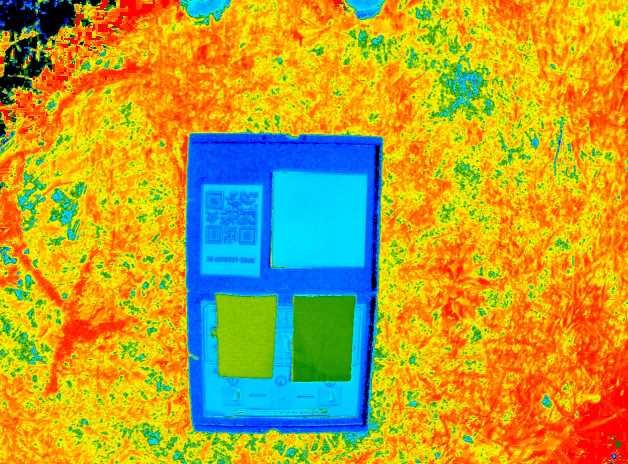
\includegraphics[scale=0.35]{images/sequoia_ndvical.jpg}
\caption{Processed NDVI from red and NIR image}
\end{subfigure}
\caption{Images taken from Parrot Sequoia}
\label{fig:cal_plate}
\end{figure}

The plate has an NDVI value of -0.088, blue paper has 0.211, and red paper has 0.085. These values seem about 75\% larger, but it is hard to quantify if it is more sensitive. Both cameras would need to be calibrated to meet the 0.18 NDVI target.\\
%0,06933333333333333333333333333333
%0.128

There does exist radiometric calibration as in Equation \ref{eq:radiometric}, however, it exists outside the scope of the project due to complexity.\\

\begin{equation}\label{eq:radiometric}
L = V(x,y)\ *\ \frac{a_1}{g}*\frac{p\ -\ p_{BL}}{t_e\ +\ a_2y\ -\ a_3t_ey}
\end{equation}

 

Where:\\
$L$ is the spectral radiance in $W/m^2/sr/nm$\\
$p$ is the raw pixel value (normalized)\\
$p_BL$ is the black level value (normalized)\\
$a1,\ a2,\ a3$ are the radiometric calibration coefficients\\
$t_e$ is the image exposure time\\
$g$ is the sensor gain setting\\
$x, y$ is the pixel column and row number\\
$V(x, y)$ is the vignette polynomial function for pixel location $(x, y)$.\\

This is part of the Parrot Sequoia calibration procedure, and it shows that more research needs to be done before the effectiveness of the Sony cameras compared to the Parrot Sequoia can be discussed.